\chapter{Top-Down Parsing}\label{ch:b3:top-down-parsing}

The \omterm{def:b3:lexical-analysis:scanner}{scanner} hands over \code{x = x * ;} as six well-formed tokens. Something must now notice that a multiplication has lost its right operand, say so at the right column, and carry on to find the next mistake rather than stop at the first. The same something must read \code{1 - 2 - 3} as $(1 - 2) - 3$ and not $1 - (2 - 3)$, which differ by 4, and \code{a + b * c} with the product inside the sum. This chapter builds the parser of Moor: a grammar, the sets that tell a parser which rule to use by looking at one token, the table those sets fill, and the hand-written parser that production compilers use, one function per rule with a loop for operators. Its output is a tree, frozen here for the rest of the book.

\section{A grammar for Moor}\label{sec:b3:top-down-parsing:grammar}

\begin{recall}
A context-free grammar has terminals, nonterminals, a start symbol and productions $A \to \alpha$. A derivation rewrites one nonterminal at a time; a leftmost derivation always rewrites the leftmost one. A parse tree records a derivation without its order; a grammar is ambiguous when some word has two parse trees. A pushdown automaton is a finite automaton with a stack, and recognises exactly the context-free languages (Year 2 volume, \emph{Context-Free Grammars and Pushdown Automata}). Rust's enums with data are sum types, and \code{match} takes them apart (Year 2 volume).
\end{recall}

A parser reads tokens and checks them against a grammar. Here is a small one for sums and products, with \code{id} standing for any identifier:
\[
E \to E + T \mid T \qquad T \to T * F \mid F \qquad F \to (\,E\,) \mid \mathit{id}.
\]
Its parse tree for \code{a + b * c} has eight interior nodes, one per rule used. Most of them carry nothing the later phases need: that $b$ was derived through $F$ and $T$ says only that it is an operand. What the compiler needs is the structure: a sum whose right operand is a product.

\begin{definition}[Abstract syntax tree]\label{def:b3:top-down-parsing:ast}
The \emph{abstract syntax tree}\index{abstract syntax tree} (AST) of a program is a tree whose nodes are the constructs of the language (an addition, a call, an \code{if} statement), each with its operands as children and its span. It omits what the grammar needed only to be unambiguous or easy to parse: parentheses, separators, the chains of nonterminals that encode precedence.
\end{definition}

\begin{omfigure}
\begin{tikzpicture}[font=\small, level distance=8mm,
  every node/.style={inner sep=1.5pt},
  nt/.style={text=omDef!80!black}, tk/.style={font=\ttfamily\small}]
  \begin{scope}
  \node[nt] {$E$}
    child {node[nt] {$E$} child {node[nt] {$T$} child {node[nt] {$F$} child {node[tk] {a}}}}}
    child {node[tk] {+}}
    child {node[nt] {$T$}
      child {node[nt] {$T$} child {node[nt] {$F$} child {node[tk] {b}}}}
      child {node[tk] {*}}
      child {node[nt] {$F$} child {node[tk] {c}}}};
  \node[font=\scriptsize] at (0,-4.3) {parse tree: 8 interior nodes};
  \end{scope}
  \begin{scope}[xshift=6.2cm, level distance=10mm, sibling distance=14mm]
  \node[draw, circle, minimum size=6mm] {$+$}
    child {node[tk] {a}}
    child {node[draw, circle, minimum size=6mm] {$*$}
      child {node[tk] {b}}
      child {node[tk] {c}}};
  \node[font=\scriptsize] at (0,-4.3) {abstract syntax tree: 2 nodes};
  \end{scope}
\end{tikzpicture}
\par\smallskip{\small The parse tree and the \omterm{def:b3:top-down-parsing:ast}{abstract syntax tree} of \code{a + b * c}. The AST keeps the operators and their operands and drops the nonterminals that only encoded precedence.}
\end{omfigure}

Moor's AST is \cref{lst:b3:top-down-parsing:ast}. An expression is a kind and a span; a statement likewise. A call names its function and an index names its array: Moor has no function values and no array values, so the thing called or indexed is always a name. The rest of the file (blocks, functions, the items of a program, and a printer that writes an expression as an S-expression such as \code{(+ a (* b c))}) follows the same pattern. Every later chapter of Part I reads this tree, and none changes it.

\omcode{code/bachelor-3/02-top-down-parsing/listings/ast.rs}{15}{43}{The expressions and statements of Moor's AST. Frozen.}\label{lst:b3:top-down-parsing:ast}

\section{Nullable, FIRST and FOLLOW}\label{sec:b3:top-down-parsing:first-follow}

A top-down parser builds the tree from the root. Facing a nonterminal $A$ and the next token $a$, it must choose a production of $A$. Three sets, computed once from the grammar, tell it which productions can possibly start with $a$.

\begin{definition}[Nullable, FIRST, FOLLOW]\label{def:b3:top-down-parsing:first-follow}
Let $G$ be a grammar and $\alpha$ a string of terminals and nonterminals. $\alpha$ is \emph{nullable}\index{nullable} if $\alpha \Rightarrow^* \varepsilon$. The \emph{FIRST set}\index{FIRST set} $\mathrm{FIRST}(\alpha)$ is the set of terminals $a$ such that $\alpha \Rightarrow^* a\beta$ for some $\beta$. For a nonterminal $A$, the \emph{FOLLOW set}\index{FOLLOW set} $\mathrm{FOLLOW}(A)$ is the set of terminals $a$ such that $S \Rightarrow^* \beta A a \gamma$ for some $\beta, \gamma$, where $S$ is the start symbol; it contains the end marker \$ if $S \Rightarrow^* \beta A$.
\end{definition}

The definitions quantify over all derivations, which are infinitely many. The sets are computed instead as the least solution of equations read off the productions. For each production $A \to X_1 \dots X_n$:
\begin{itemize}
\item $A$ is \omterm{def:b3:top-down-parsing:first-follow}{nullable} if every $X_i$ is;
\item $\mathrm{FIRST}(A) \supseteq \mathrm{FIRST}(X_i)$ whenever $X_1 \dots X_{i-1}$ is \omterm{def:b3:top-down-parsing:first-follow}{nullable} (and $\mathrm{FIRST}(a) = \{a\}$ for a terminal);
\item for each nonterminal $X_i$, $\mathrm{FOLLOW}(X_i)$ contains $\mathrm{FIRST}(X_{i+1} \dots X_n)$, and also $\mathrm{FOLLOW}(A)$ if $X_{i+1} \dots X_n$ is \omterm{def:b3:top-down-parsing:first-follow}{nullable}.
\end{itemize}

\begin{method}[Sets by iteration]\label{met:b3:top-down-parsing:iterate}
Start with every set empty and no nonterminal \omterm{def:b3:top-down-parsing:first-follow}{nullable}, and $\$ \in \mathrm{FOLLOW}(S)$. Pass over the productions, applying each inclusion above and growing the sets; repeat until a whole pass changes nothing. Do \omterm{def:b3:top-down-parsing:first-follow}{nullable} and FIRST first, then FOLLOW, which needs them.
\end{method}

Each pass can only add, and the sets are bounded by the number of terminals, so the iteration stops; what it computes is the least solution, the one the definitions describe (exercise~\ref{exo:b3:top-down-parsing:7}). Chapter~8 meets this pattern again, as a fixed point of dataflow equations. \Cref{lst:b3:top-down-parsing:compute} is the method over a grammar read from a text file.

\omcode{code/bachelor-3/02-top-down-parsing/listings/grammar.rs}{68}{106}{\omterm{def:b3:top-down-parsing:first-follow}{Nullable}, FIRST and FOLLOW as least fixed points. \code{first_seq} computes FIRST of a sequence and tells whether it is \omterm{def:b3:top-down-parsing:first-follow}{nullable}.}\label{lst:b3:top-down-parsing:compute}

The grammar of sums and products above cannot be parsed top-down as it stands, for a reason the next section gives. Here it is rewritten into an equivalent one that can, and its sets.

\omcode{code/bachelor-3/02-top-down-parsing/listings/expr.grammar}{1}{6}{Sums and products, with \omterm{def:b3:top-down-parsing:left-recursion}{left recursion} removed: $E'$ is ``the rest of a sum''.}\label{lst:b3:top-down-parsing:exprgrammar}
\omoutput{code/bachelor-3/02-top-down-parsing/outputs/first_follow.txt}{\omterm{def:b3:top-down-parsing:first-follow}{Nullable}, FIRST and FOLLOW of \cref{lst:b3:top-down-parsing:exprgrammar}.}\label{out:b3:top-down-parsing:sets}

Read the \omterm{def:b3:top-down-parsing:first-follow}{FOLLOW sets} as ``what may come after''. A product $T$ may be followed by \code{+} (more sum), by \code{)} (the end of a parenthesised sum) or by the end of input. A factor $F$ may in addition be followed by \code{*}.

\section{LL(1) grammars}\label{sec:b3:top-down-parsing:ll1}

\begin{definition}[LL(1) grammar, predictive parsing table]\label{def:b3:top-down-parsing:ll1}
The \emph{predictive parsing table}\index{predictive parsing table} of a grammar has a row per nonterminal and a column per terminal (and \$). Production $A \to \alpha$ is put in cell $[A, a]$ for every $a \in \mathrm{FIRST}(\alpha)$, and, if $\alpha$ is \omterm{def:b3:top-down-parsing:first-follow}{nullable}, for every $a \in \mathrm{FOLLOW}(A)$. A grammar is an \emph{LL(1) grammar}\index{LL(1) grammar} if no cell of its table holds two productions.
\end{definition}

The name says how such a grammar is parsed: from Left to right, building a Leftmost derivation, with 1 token of lookahead. Equivalently, for any two productions $A \to \alpha \mid \beta$: $\mathrm{FIRST}(\alpha)$ and $\mathrm{FIRST}(\beta)$ are disjoint, at most one of them is \omterm{def:b3:top-down-parsing:first-follow}{nullable}, and if $\beta$ is \omterm{def:b3:top-down-parsing:first-follow}{nullable} then $\mathrm{FIRST}(\alpha)$ and $\mathrm{FOLLOW}(A)$ are disjoint.

\begin{method}[The predictive parser]\label{met:b3:top-down-parsing:predictive}
Keep a stack of grammar symbols, initially \$ below the start symbol, and the input followed by \$. Repeat: if the top is a terminal, it must equal the next input token; pop it and advance. If the top is a nonterminal $A$ and the next token is $a$, look up $[A, a]$: if it is empty, report an error; otherwise pop $A$ and push the production's right side, its first symbol on top. Accept when both the stack and the input are down to \$.
\end{method}

This is a pushdown automaton whose transitions are read from the table. \Cref{out:b3:top-down-parsing:driver} runs it on \code{id + id * id}, and the figure after it draws the first stacks.

\omoutput{code/bachelor-3/02-top-down-parsing/outputs/ll1_driver.txt}{The predictive parser of \cref{lst:b3:top-down-parsing:exprgrammar} on \code{id + id * id}: each line shows the stack, the input left, and what the table said.}\label{out:b3:top-down-parsing:driver}

\begin{omfigure}
\begin{tikzpicture}[font=\scriptsize, x=12mm,
  cel/.style={draw, minimum width=9mm, minimum height=4.5mm, inner sep=0pt, fill=omDef!6}]
  \foreach \col/\items/\lab in {0/{\$,E}/start, 1/{\$,E',T}/{$E \to T E'$}, 2/{\$,E',T',F}/{$T \to F T'$},
                                3/{\$,E',T',id}/{$F \to id$}, 4/{\$,E',T'}/{match id}, 5/{\$,E'}/{$T' \to \varepsilon$},
                                6/{\$,E',T,+}/{$E' \to + T E'$}, 7/{\$,E',T}/{match +}} {
    \foreach \s [count=\k from 0] in \items
      \node[cel] at (\col*1.05, \k*0.5) {\s};
    \node[anchor=north, align=center, text width=11mm] at (\col*1.05, -0.4) {\lab};
  }
\end{tikzpicture}
\par\smallskip{\small The first eight stacks of the predictive parser, bottom to top: each column is the stack after the action written under it. Predicting a production replaces a nonterminal by its right side; matching pops a terminal.}
\end{omfigure}

\begin{theorem}[Predictive parsing is correct for LL(1) grammars]\label{thm:b3:top-down-parsing:ll1}
If $G$ is LL(1), the predictive parser accepts a word $w$ if and only if $w \in L(G)$, and then the productions it predicts, in order, are those of the leftmost derivation of $w$.
\end{theorem}

\begin{proof}
At every step the stack, read from top to bottom, is a sentential form $\gamma$ such that $S \Rightarrow^*_{\mathrm{lm}} u\gamma$ where $u$ is the input already matched: this holds at the start ($u = \varepsilon$, $\gamma = S$), and each prediction or match keeps it. So an accepted word is derived by the predicted productions, leftmost first. Conversely, let $w \in L(G)$ with leftmost derivation $D$. Suppose the parser has followed $D$ so far and $D$ next rewrites the top nonterminal $A$ by $A \to \alpha$, with $a$ the next token. Either $\alpha$ derives a word starting with $a$, so $a \in \mathrm{FIRST}(\alpha)$, or $\alpha$ derives $\varepsilon$ in $D$ and $a$ comes from what follows $A$, so $a \in \mathrm{FOLLOW}(A)$ and $\alpha$ is \omterm{def:b3:top-down-parsing:first-follow}{nullable}. Either way $A \to \alpha$ is in cell $[A, a]$, and it is alone there because $G$ is LL(1): the parser predicts the production of $D$. By induction it follows $D$ to the end and accepts.
\end{proof}

Two features of grammars put two productions in one cell. The first is the one that made $E \to E + T$ unusable.

\begin{definition}[Left recursion, left factoring]\label{def:b3:top-down-parsing:left-recursion}
A grammar has \emph{left recursion}\index{left recursion} if some nonterminal $A$ derives $A\alpha$ in one or more steps. \emph{Left factoring}\index{left factoring} replaces productions $A \to \beta\gamma_1 \mid \beta\gamma_2$ that share a prefix $\beta$ by $A \to \beta A'$ and $A' \to \gamma_1 \mid \gamma_2$, with a new nonterminal $A'$.
\end{definition}

A left-recursive production $A \to A\alpha \mid \beta$ puts both productions in every cell of $\mathrm{FIRST}(\beta)$: whatever starts a $\beta$ also starts an $A\alpha$. The standard rewrite replaces it by $A \to \beta A'$ and $A' \to \alpha A' \mid \varepsilon$, which generates the same words, $\beta\alpha^*$, from the left; \cref{lst:b3:top-down-parsing:exprgrammar} is that rewrite applied twice. \omterm{def:b3:top-down-parsing:left-recursion}{Left factoring} handles the second problem. A Moor statement can be \code{x = e;} or an expression \code{e;}, and both can start with an identifier. \Cref{out:b3:top-down-parsing:table} prints the table of a small grammar with exactly that conflict, before and after factoring out the common \code{id}.

\omoutput{code/bachelor-3/02-top-down-parsing/outputs/ll1_table.txt}{The table of \code{S -> id = E ; | E ;} (one conflict), and of its left-factored form, which is LL(1).}\label{out:b3:top-down-parsing:table}

The whole of Moor can be written as an \omterm{def:b3:top-down-parsing:ll1}{LL(1) grammar}: \code{moor.grammar} in this chapter's listings does it in 37 nonterminals, and its table of 278 cells has no conflict (the tests check it). But the factoring needed for statements spreads through every precedence level: after \code{x} has been read as the start of an expression statement, the grammar needs a nonterminal for ``the rest of an expression whose first operand was a name'', which is the tail of a product, then of a sum, of a comparison, and so on up to \code{||}. Nobody writes a parser from that grammar by hand. The parser of the next section reads one token further instead.

\begin{history}[LL and Pratt]
Philip Lewis and Richard Stearns defined the LL($k$) grammars in July 1968, in a paper on syntax-directed translation. % ledger: b3:lewis-stearns-1968
Vaughan Pratt presented ``top down operator precedence'' at the first Principles of Programming Languages symposium in 1973: a parser in which each token carries its own \omterm{def:b3:top-down-parsing:precedence}{binding power}, the method this chapter calls \omterm{def:b3:top-down-parsing:precedence}{precedence climbing}. % ledger: b3:pratt-1973
\end{history}

\section{Recursive descent}\label{sec:b3:top-down-parsing:descent}

\begin{definition}[Recursive descent]\label{def:b3:top-down-parsing:descent}
A \emph{recursive descent}\index{recursive descent} parser has one function per nonterminal. The function for $A$ looks at the next token (or the next few), chooses a production of $A$, and runs through its right side: it consumes each terminal and calls the function of each nonterminal. The call stack of the program plays the part of the parser's stack.
\end{definition}

The function for a Moor function definition is \cref{lst:b3:top-down-parsing:func}: it follows the production \code{fn id ( params ) [-> type] block} symbol by symbol, with a loop where the grammar has a repetition.

\omcode{code/bachelor-3/02-top-down-parsing/listings/parser.rs}{164}{188}{\omterm{def:b3:top-down-parsing:descent}{Recursive descent} for a function definition: each line is one symbol of the production.}\label{lst:b3:top-down-parsing:func}

Where Moor is not LL(1) as written, the parser looks two tokens ahead. An identifier followed by \code{=} starts an assignment; anything else starts an expression. An assignment to an array element, \code{a[i] = e;}, is found differently: the parser reads an expression, and if an \code{=} follows, checks that the expression it read was an element. This ``parse, then check the target'' is how most hand-written parsers handle assignment, and it gives a better message for \code{f(x) = 1;} than a grammar could.

\omcode{code/bachelor-3/02-top-down-parsing/listings/parser.rs}{282}{306}{The end of the statement function: two-token lookahead for \code{x = e;}, and the check of an assignment's target.}\label{lst:b3:top-down-parsing:stmt}

Expressions are where the classic layout of \omterm{def:b3:top-down-parsing:descent}{recursive descent} is wasteful. With one function per precedence level, as the grammar of sums and products suggests, a single number in a Moor condition goes through eight calls: \code{||}, \texttt{\&\&}, equality, comparison, sum, product, prefix, and primary, each finding no operator of its own and returning. \omterm{def:b3:top-down-parsing:precedence}{Precedence climbing} replaces all the levels by one function and a table.

\begin{definition}[Binding power, precedence climbing]\label{def:b3:top-down-parsing:precedence}
The \emph{binding power}\index{binding power} of a binary operator is a positive integer, higher for operators that bind more tightly: in Moor, 1 for \code{||}, 2 for \texttt{\&\&}, 3 for \code{==} and \code{!=}, 4 for the comparisons, 5 for \code{+} and \code{-}, 6 for \code{*}, \code{/} and \texttt{\%}. \emph{Precedence climbing}\index{precedence climbing} parses an expression whose operators all have binding power at least $m$ as follows: parse an operand; then, while the next token is an operator of power $p \ge m$, consume it, parse the right operand as an expression of minimum power $p + 1$, and combine.
\end{definition}

\omcode{code/bachelor-3/02-top-down-parsing/listings/parser.rs}{332}{356}{\omterm{def:b3:top-down-parsing:precedence}{Precedence climbing} and the prefix operators. \code{bp + 1} makes every binary operator left-associative.}\label{lst:b3:top-down-parsing:climb}

\begin{theorem}[Precedence climbing respects the table]\label{thm:b3:top-down-parsing:climb}
In the tree that \code{expr_bp(1)} builds from operands and binary operators, every operator node of power $p$ has a left child of power at least $p$ and a right child of power greater than $p$ (an operand counts as power $\infty$). So operators of higher power are deeper, and operators of equal power group to the left.
\end{theorem}

\begin{proof}
A call \texttt{expr\_bp($m$)} returns a tree all of whose operators have power at least $m$: it only combines operators with $p \ge m$, and their right operands come from calls with minimum $p + 1 > m$; this is an induction on the depth of calls. Now take a node built by the loop for an operator of power $p$. Its right child came from \texttt{expr\_bp($p + 1$)}, so its root has power at least $p + 1$. Its left child is the tree built so far in the same call: either the first operand, or a node for an operator $q$ combined earlier in the same loop. When the loop combined $q$, the right operand of $q$ stopped at our operator, so $p < q + 1$, that is $q \ge p$.
\end{proof}

\omoutput{code/bachelor-3/02-top-down-parsing/outputs/prec_demo.txt}{Trees built by \omterm{def:b3:top-down-parsing:precedence}{precedence climbing}. The last expression is refused: Moor indexes only a name, not the result of a call.}\label{out:b3:top-down-parsing:prec}

The figure below compares the calls of the two layouts on \code{a + b * c}. \omterm{def:b3:top-down-parsing:precedence}{Precedence climbing} makes a call per operand and a call per operator's right side; the layered parser makes a call per level for each operand, whether or not an operator of that level appears.

\begin{omfigure}
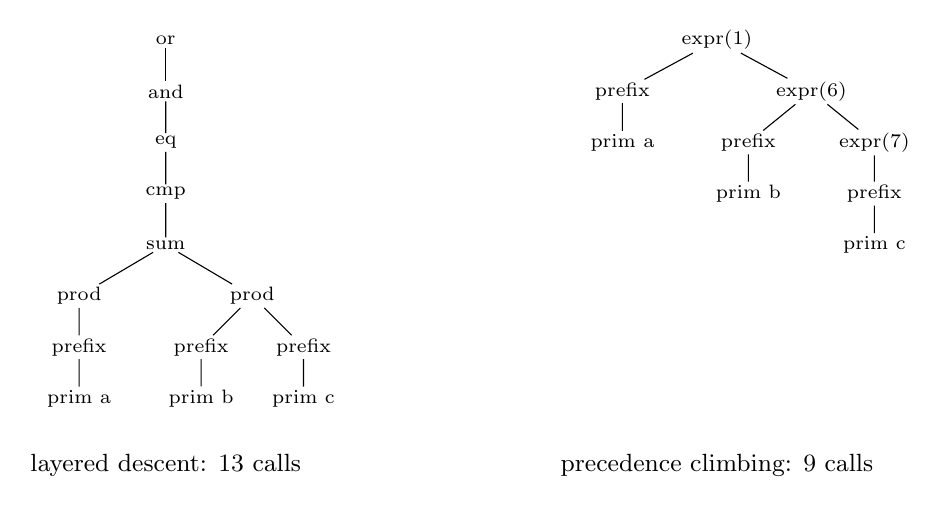
\begin{tikzpicture}[font=\scriptsize, level distance=6.5mm, sibling distance=9mm,
  every node/.style={inner sep=1pt}]
  \node {or} child {node {and} child {node {eq} child {node {cmp} child {node {sum}
      child[sibling distance=22mm] {node {prod} child {node {prefix} child {node {prim a}}}}
      child[sibling distance=22mm] {node {prod}
         child[sibling distance=13mm] {node {prefix} child {node {prim b}}}
         child[sibling distance=13mm] {node {prefix} child {node {prim c}}}}}}}};
  \node[font=\small] at (0,-5.4) {layered descent: 13 calls};
  \begin{scope}[xshift=7cm]
  \node {expr(1)}
    child[sibling distance=24mm] {node {prefix} child {node {prim a}}}
    child[sibling distance=24mm] {node {expr(6)}
      child[sibling distance=16mm] {node {prefix} child {node {prim b}}}
      child[sibling distance=16mm] {node {expr(7)} child {node {prefix} child {node {prim c}}}}};
  \node[font=\small] at (0,-5.4) {precedence climbing: 9 calls};
  \end{scope}
\end{tikzpicture}
\par\smallskip{\small Call trees for \code{a + b * c}. Left: one function per level of \code{||}, \texttt{\&\&}, equality, comparison, sum, product, then the prefix operators and the primary. Right: the parser of \cref{lst:b3:top-down-parsing:climb}, where the right side of \code{+} is parsed with minimum power 6 and that of \code{*} with 7.}
\end{omfigure}

\Cref{out:b3:top-down-parsing:fib} runs the whole parser on the Fibonacci program and prints its tree, one statement per line.

\omcode{code/bachelor-3/02-top-down-parsing/listings/fib.moor}{2}{10}{\texttt{fib.moor}.}\label{lst:b3:top-down-parsing:fib}
\omoutput{code/bachelor-3/02-top-down-parsing/outputs/parse_demo.txt}{The \omterm{def:b3:top-down-parsing:ast}{abstract syntax tree} of \texttt{fib.moor}.}\label{out:b3:top-down-parsing:fib}

\section{Recovering from errors}\label{sec:b3:top-down-parsing:recovery}

A parser that stops at the first error makes its user fix one mistake per compilation. A parser that carries on blindly reports a cascade of errors that are all the first one in disguise. The usual compromise is cheap and works well.

\begin{definition}[Panic-mode recovery, synchronising token]\label{def:b3:top-down-parsing:recovery}
In \emph{panic-mode recovery}\index{panic-mode recovery}, a parser that meets an error records it, then skips tokens until it reaches a \emph{synchronising token}\index{synchronising token}: a token after which parsing can resume in a known state. It then resumes from the function that handles that state.
\end{definition}

In Moor, a statement ends at \code{;}, and \code{var}, \code{if}, \code{while}, \code{return} and \texttt{\}} begin or end one: these are the \omterm{def:b3:top-down-parsing:recovery}{synchronising tokens} for statements. A statement function that fails returns an error marker up to the block function, which calls \cref{lst:b3:top-down-parsing:sync} and then tries the next statement. At the top level, \code{fn}, \code{var} and \code{array} play the same part.

\omcode{code/bachelor-3/02-top-down-parsing/listings/parser.rs}{236}{251}{Panic mode: skip to the end of the statement, or to the start of the next one.}\label{lst:b3:top-down-parsing:sync}

\omcode{code/bachelor-3/02-top-down-parsing/listings/errors.moor}{1}{6}{Three syntax errors.}\label{lst:b3:top-down-parsing:errors}
\omoutput{code/bachelor-3/02-top-down-parsing/outputs/recover.txt}{All three are reported, each once, and the tree is built for the rest.}\label{out:b3:top-down-parsing:recover}

The third error shows a limit: the missing semicolon is after \code{print(x)}, but the parser can only notice it at the \texttt{\}} that follows. An error is always reported where the parser first finds the input impossible, which may be after the mistake. Panic mode also loses whatever a skipped region contained, so an error inside a skipped region goes unreported until the next compilation.

\begin{inpractice}[Error messages are part of the language]
The messages of \cref{out:b3:top-down-parsing:recover} name what was expected and what was found, and point at a column. That is most of what a programmer needs. Production parsers add two things: a guess at the fix when one is likely (``missing \code{;}?''), and care to report an error once even when several functions notice it. Both are easier in a hand-written parser than in a generated one, which is the main reason most compilers of widely used languages parse by \omterm{def:b3:top-down-parsing:descent}{recursive descent}.
\end{inpractice}

\section{Exercises}\label{sec:b3:top-down-parsing:exercises}

\begin{exercise}[$\star$]\label{exo:b3:top-down-parsing:1}
Compute \omterm{def:b3:top-down-parsing:first-follow}{nullable} and FIRST for the grammar $S \to A\,B\,c \mid d$, $A \to a\,A \mid \varepsilon$, $B \to b \mid \varepsilon$.
\end{exercise}

\begin{exercise}[$\star$]\label{exo:b3:top-down-parsing:2}
Write the S-expression that the parser of this chapter builds for \texttt{a - -b * c \% d || !e}.
\end{exercise}

\begin{exercise}[$\star$]\label{exo:b3:top-down-parsing:3}
Is the grammar $S \to A\,a \mid b$, $A \to a \mid \varepsilon$ LL(1)? Fill its table and say which cell decides. Describe the language it generates and give an \omterm{def:b3:top-down-parsing:ll1}{LL(1) grammar} for it.
\end{exercise}

\begin{exercise}[$\star$]\label{exo:b3:top-down-parsing:4}
Remove the \omterm{def:b3:top-down-parsing:left-recursion}{left recursion} from $L \to L\,,\,\mathit{id} \mid \mathit{id}$ (a comma-separated list), and write the recursive-descent function for the result as a loop.
\end{exercise}

\begin{exercise}[$\star\star$]\label{exo:b3:top-down-parsing:5}
\Cref{lst:b3:top-down-parsing:minus} is a calculator for one-digit numbers. Three of its five answers in \cref{out:b3:top-down-parsing:minus} are wrong. Find the bug, explain the wrong answers, and fix it.
\omcode{code/bachelor-3/02-top-down-parsing/listings/minus_bug.rs}{10}{30}{A calculator by \omterm{def:b3:top-down-parsing:precedence}{precedence climbing}.}\label{lst:b3:top-down-parsing:minus}
\omoutput{code/bachelor-3/02-top-down-parsing/outputs/minus_bug.txt}{Its answers.}\label{out:b3:top-down-parsing:minus}
\end{exercise}

\begin{exercise}[$\star\star$]\label{exo:b3:top-down-parsing:6}
Add to \code{moor.grammar} a loop \texttt{for i = a to b \{ \dots\ \}}, with an optional \code{step c} before the block, and check with the chapter's tools that the grammar stays LL(1). Then say how a parser can build this loop from the existing AST nodes alone, and which choice the language designer must make about \code{b}.
\end{exercise}

\begin{exercise}[$\star\star$]\label{exo:b3:top-down-parsing:7}
Prove that \cref{met:b3:top-down-parsing:iterate} terminates, after at most $|N|\,(|T| + 1) + 1$ passes for FOLLOW, where $N$ and $T$ are the sets of nonterminals and terminals, and that the sets it computes are the least ones satisfying the inclusions. Then prove that the least solution is the FOLLOW of the definition.
\end{exercise}

\begin{exercise}[$\star\star$]\label{exo:b3:top-down-parsing:8}
Predict the messages, with line and column, of the parser on this file (lines numbered from 1), and say what panic mode skips after each:
\omcode{code/bachelor-3/02-top-down-parsing/exercises/ex8.moor}{1}{5}{A file with mistakes.}\label{lst:b3:top-down-parsing:ex8}
\end{exercise}

\begin{exercise}[$\star\star$]\label{exo:b3:top-down-parsing:9}
Count the calls the parser of \cref{lst:b3:top-down-parsing:climb} makes (of \code{expr_bp}, \code{prefix} and \code{primary}) on a chain of $n$ operands joined by \code{+}, and the calls a layered recursive-descent parser makes (one function per level as in the figure of call trees). Do the same for a chain of products.
\end{exercise}

\begin{exercise}[$\star\star\star$]\label{exo:b3:top-down-parsing:10}
Prove that an \omterm{def:b3:top-down-parsing:ll1}{LL(1) grammar} is unambiguous. Is the converse true?
\end{exercise}

\begin{exercise}[$\star\star\star$]\label{exo:b3:top-down-parsing:11}
Show that the grammar $S \to A \mid B$, $A \to a\,A\,b \mid c$, $B \to a\,B\,b\,b \mid d$ is not LL($k$) for any $k$: no fixed number of tokens of lookahead lets a top-down parser choose between $A$ and $B$. Give a parser that does recognise its language by reading the input once, and say why it is not top-down in the sense of this chapter.
\end{exercise}

\begin{exercise}[$\star\star\star$]\label{exo:b3:top-down-parsing:12}
Some languages let the programmer declare new operators with a precedence and an associativity. Write a precedence-climbing parser whose operator table is given at run time: each operator has a \omterm{def:b3:top-down-parsing:precedence}{binding power} and is left-associative, right-associative, or non-associative (\code{a == b == c} is then an error). Test it on a table with a right-associative power and a list constructor \code{::}.
\end{exercise}

\section{Weekend problem}\label{sec:b3:top-down-parsing:problem}

\begin{problem}[{Weekend problem --- The library's fines formula}]\label{pb:b3:top-down-parsing:1}
Brenmoor's library computes a late fine with a formula typed by a clerk, for instance
\begin{center}\small\ttfamily max(0, days - 14) * rate + 2 \textasciicircum{} late \textasciicircum{} 2 * (items > 3)\\ + 10 * (lost or damaged and items >= 1)\end{center}
Formulas have numbers, names, calls \texttt{max(\dots)} and \texttt{min(\dots)}, parentheses, and seven levels of binary operators, loosest first: \code{or}; \code{and}; \code{==} \code{!=}; \code{<} \code{<=} \code{>} \code{>=}; \code{+} \code{-}; \code{*} \code{/}; and \texttt{\textasciicircum}, the power, which is right-associative. The file \code{exercises/pb_fines.rs} parses formulas in two ways and counts the calls; reason each answer out before running it.

\medskip\noindent\textbf{Part I --- The grammar.}
\begin{enumerate}
\item Write a grammar for formulas with one nonterminal per level, in the style $E \to E + T \mid T$. Which productions are left-recursive, and which one is right-recursive, and why?
\item Remove the \omterm{def:b3:top-down-parsing:left-recursion}{left recursion}, as in \cref{lst:b3:top-down-parsing:exprgrammar}. How many nonterminals does the result have?
\item The power level is $P \to U\,\textasciicircum\,P \mid U$. Left-factor it.
\item A name may be followed by \code{(} for a call. Write the productions of the primary so that the grammar stays LL(1).
\item Draw the \omterm{def:b3:top-down-parsing:ast}{abstract syntax tree} of \texttt{2 \textasciicircum{} late \textasciicircum{} 2 * (items > 3)}.
\item What is the value of the example formula for days 20, rate 3, late 1, items 4, lost 0 and damaged 1 (\code{and} and \code{or} give 1 or 0)?
\end{enumerate}

\medskip\noindent\textbf{Part II --- Sets and table.}
\begin{enumerate}[resume]
\item Compute FIRST of the primary and of every level's nonterminal. Why are they all equal?
\item Compute FOLLOW of the primary, and of the ``rest of a sum'' nonterminal.
\item Fill the row of the ``rest of a sum'' nonterminal in the table. Which columns hold its $\varepsilon$-production?
\item Check that the grammar is LL(1) with \code{grammar.rs}.
\item The clerk asks for the unary minus \code{-x}. Add it at the right level and check that the grammar stays LL(1).
\item Would a comparison chain \code{a < b < c} parse? What does it mean with 0 and 1 as truth values, and should the grammar allow it?
\end{enumerate}

\medskip\noindent\textbf{Part III --- Recursive descent, counted.}
\begin{enumerate}[resume]
\item The layered parser has a function per level plus one for the primary: $p + 1 = 8$ functions. Show that the function of level $k$ (from 0, loosest) is called $1 + \sum_{j < k} o_j$ times on a formula without parentheses, calls or powers, where $o_j$ is the number of operators of level $j$.
\item Deduce the number of calls on a chain of $n$ operands joined by \code{or}, by \code{+}, and by \texttt{\textasciicircum}.
\item Which chain is the worst case for a fixed $n$, and how many calls does it take with $p$ levels?
\item How are parentheses and the arguments of a call counted?
\item Count the calls on the example formula, and check with the program.
\item Where does the time go: how many of these calls find no operator of their own level?
\end{enumerate}

\medskip\noindent\textbf{Part IV --- Precedence climbing.}
\begin{enumerate}[resume]
\item Give the \omterm{def:b3:top-down-parsing:precedence}{binding powers} that make \omterm{def:b3:top-down-parsing:precedence}{precedence climbing} build the same trees, and say what the right-associative power changes in the recursive call.
\item Show that \omterm{def:b3:top-down-parsing:precedence}{precedence climbing} makes exactly two calls per primary: one to parse the primary and one to parse an expression that starts with it, or the whole formula.
\item Count its calls on the three chains of question 14 and on the example formula.
\item The program parses 2,000 random formulas both ways. What must it check, and why is that enough to trust the counts?
\item Adding an eighth level to the language: what does it cost each parser, per primary?
\item State the result: calls of each parser on a chain of $n$ operands at the loosest level with $p$ levels, and on the example formula.
\end{enumerate}
\end{problem}
